\documentclass{article}
\usepackage[utf8]{inputenc}
\usepackage{graphicx}
\usepackage{geometry}
\usepackage{amsmath}
\usepackage{amsfonts}
\usepackage{float}
\usepackage{caption}
\usepackage{subcaption}
\usepackage{enumitem}

\geometry{left=25mm, top=25mm, right=25mm, bottom=25mm}

\title{PHY407 Lab 7}
\author{Pierino Zindel (1002429703) and Hayden Johnson (1002103537)}
\date{October 26, 2018}

\begin{document}

\maketitle

\noindent \textbf{Distribution of work:} Question 1 was completed by Pierino. Question 2 was completed by Hayden.

\section{Return of the Space Garbage}

The objective of this question is to take the solution of the orbital trajectories modeled in Lab 06 and implement an adaptive time step to use with 4th order Runge-Kutta to compare to the previous results.

\subsection{Part a)}
We implement a variable time step by setting our initial step size to be $h=0.01s$ and error per step size to be $\delta=10^{-6}$. We then proceed by computing the position values after two steps of size $h$ and the position values after one step of size $2h$. The position values are then used to compute the $\rho$ value using the equation

\begin{equation}
	\rho = \frac{h\delta}{sqrt(\epsilon_x^2 + \epsilon_y^2)}
\end{equation}
with 
\begin{equation}
	\epsilon_i = \frac{(i_1-i_2)}{30}
\end{equation}
for $i=x,y$.
The step size $h$ is then updated via $h\prime = h\rho^{1/4}$ and if $\rho$ is determined to be within our desired threshold the position values are recorded and we repeat the computations at time $t+2h$. If $\rho$ is outside of the threshold we use recalculate the positions of two steps and one double step for the updated $h$ value and again update $\rho$ and $h$ to determine if the error is small enough.

This is repeated for the desired number of steps $N=1000$ and plotted overlying of the results we got in Lab 06. The plot is shown in figure \ref{fig:q1_a} and from it we can see the effects of the adaptive time step based on the spacing of the dots. We can intuit that based on Kepler's laws the ball bearing will be traveling faster at perihelion than at aphelion. Thus the changes in position for a given time frame will be greater close to the rod than further away from it. As a result our adaptive time step program uses a greater number of smaller magnitude time steps when the orbit takes the ball bearing closer to the rod and a lower number of greater magnitude time steps when the orbit bring the ball far from the rod. Comparing this to the fixed time step solution underneath we can also see that the adaptive step program is more efficient and is capable of computing a larger time range using the same number of steps. 

\begin{figure}[H]
	\centering
	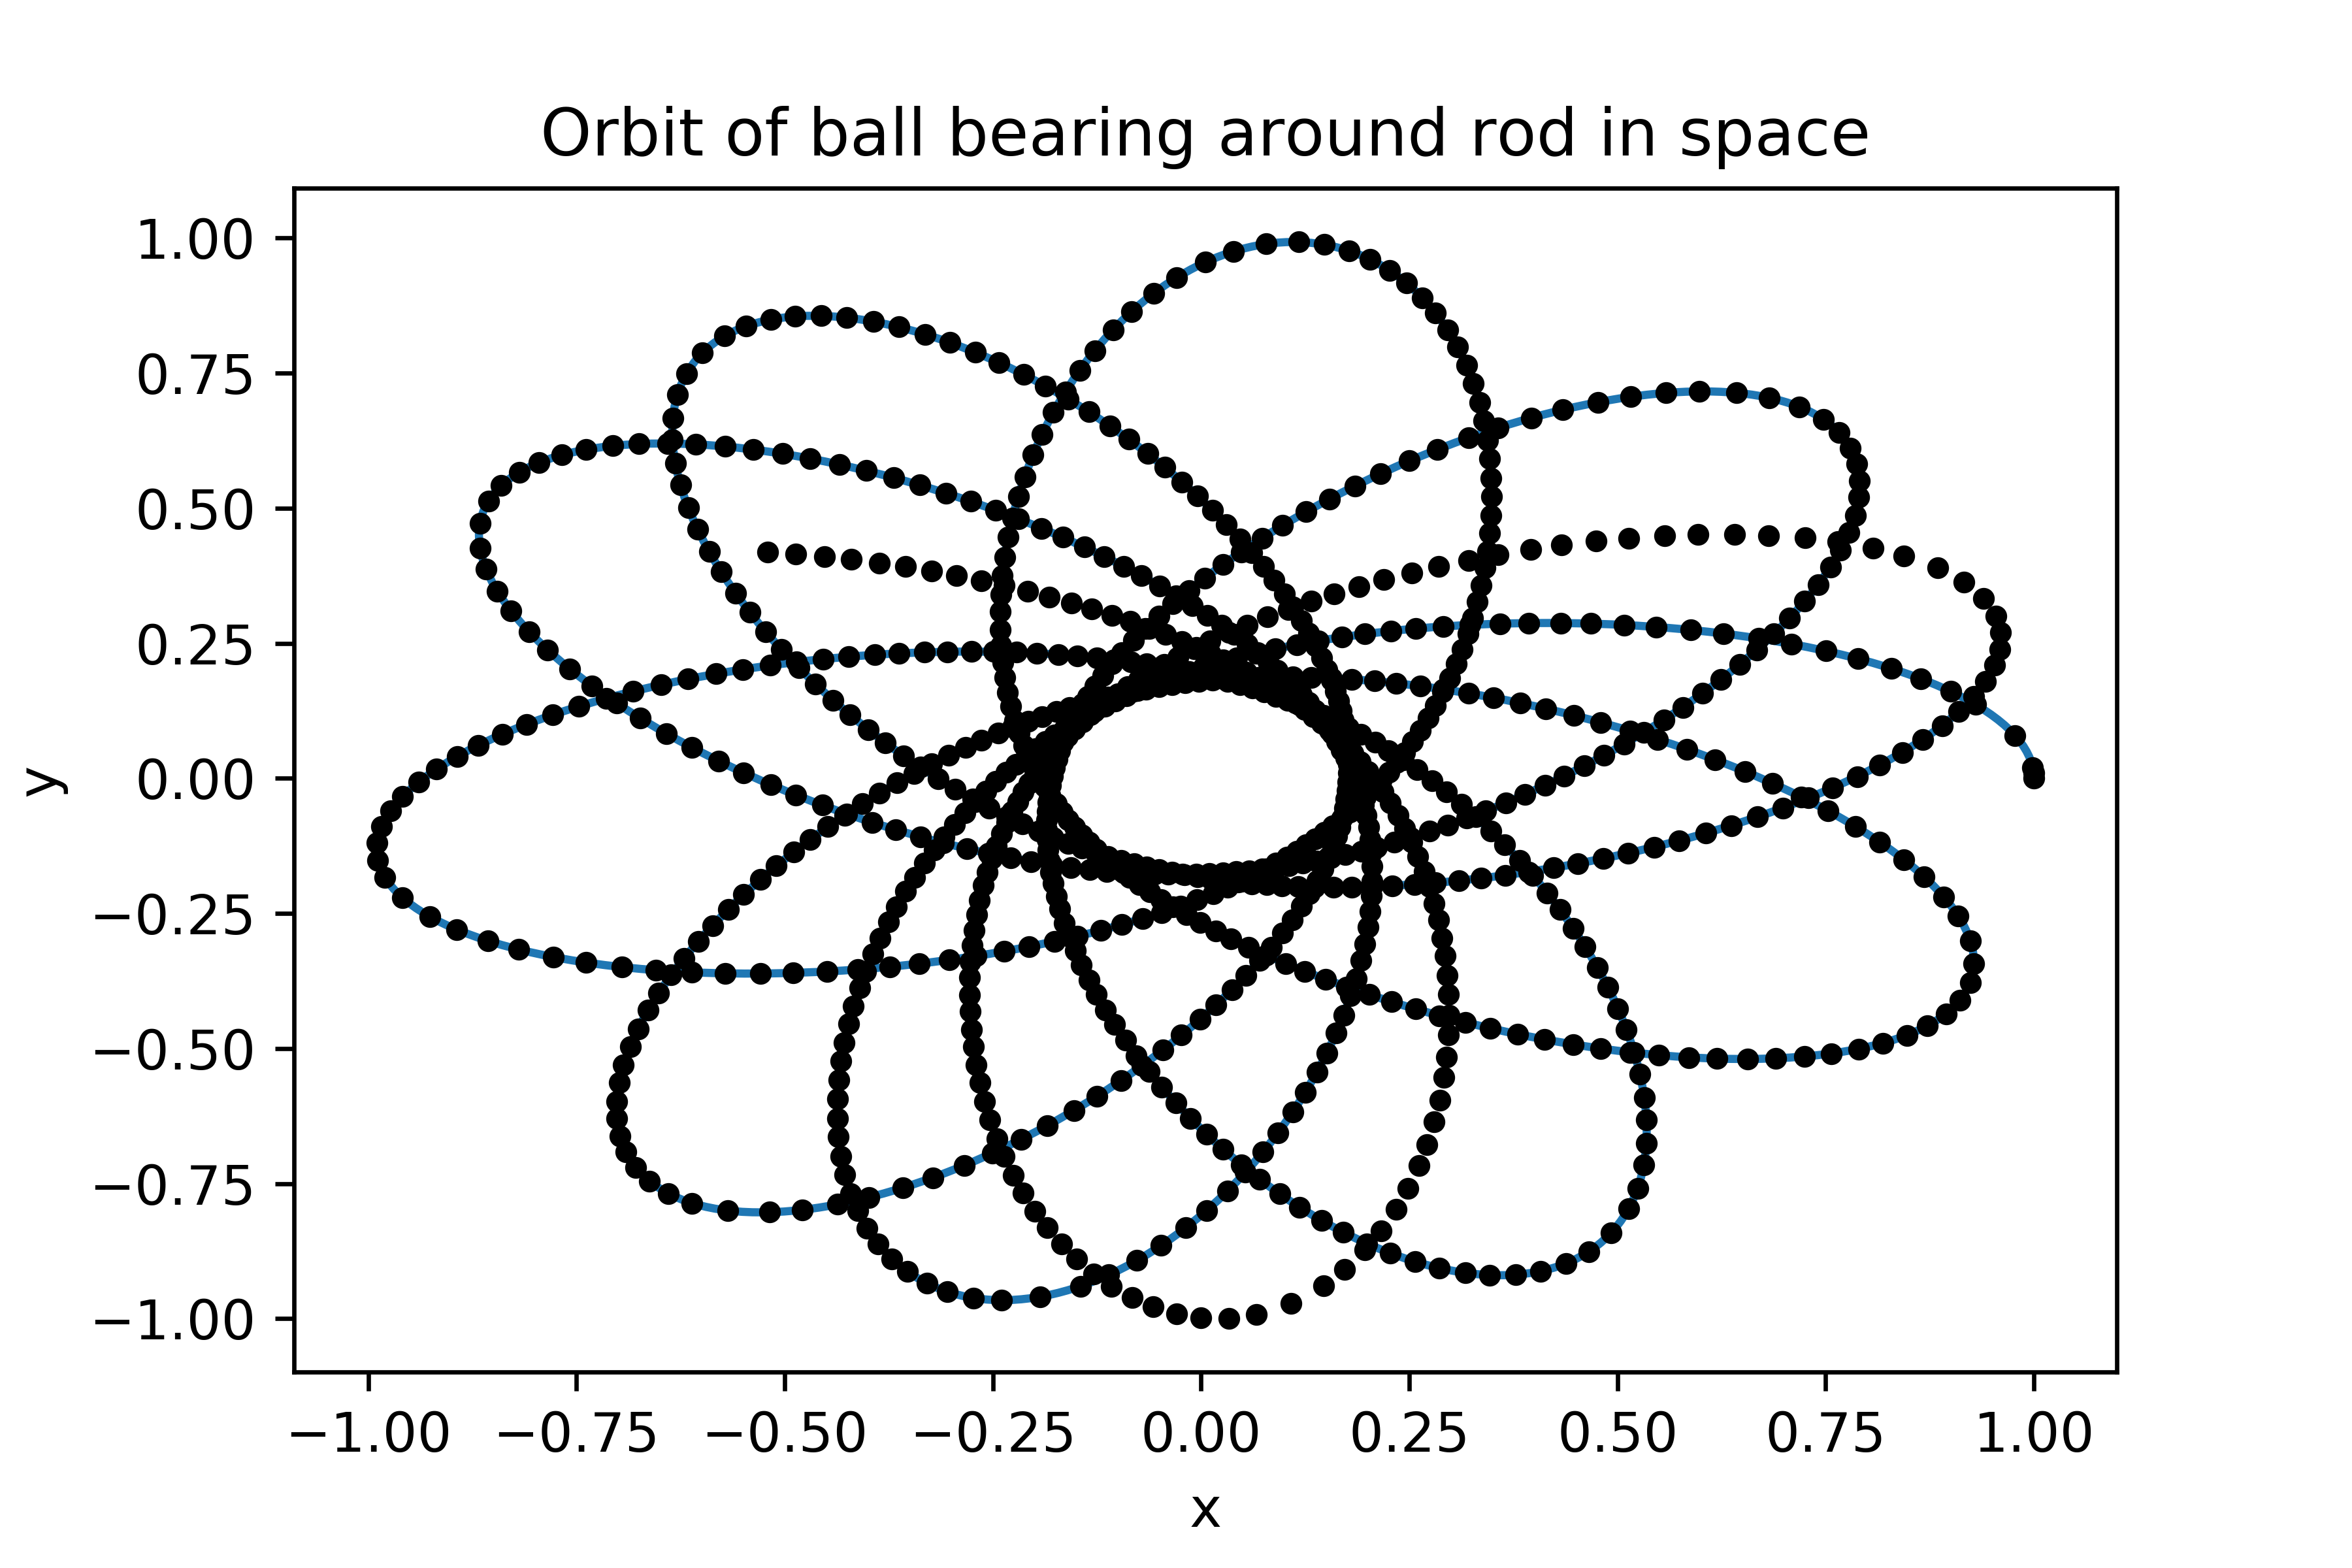
\includegraphics[width=0.8\textwidth]{../images/q1_orbit.png}
	\caption{Orbit of a ball bearing in space rotating around a rod in a plane perpendicular to the axis of the rod. The black dots are the points computed using an adaptive time step, overlying the curve corresponding to the solution computed using a fixed time step.}
	\label{fig:q1_a}
\end{figure}

\subsection{Part b)}
We now wish to compare the computation times of the fixed step method with the adaptive step method. Running the fixed step method with a step size of $h=0.01s$ for $N=1000$ steps yields a total computation time of $t=0.06249s$. The same fixed step method with a step size of $h=0.001s$ for $N=10,000$ steps yields a total computation time of $t=0.5404s$.
Comparatively, the adaptive step method with an initial step size of $h=0.01s$ for $N=1000$ steps yields a total computation time of $t=0.1562s$ while the adaptive step method with an initial step size of $h=0.001s$ for $N=10,000$ steps yields a total computation time of $t=1.523s$.

From this we can see that the using the same number of steps the adaptive step method takes at least 2 to 3 times longer. We can estimate that the reasons for this is due to the adaptive step method additionally computing the solution at every other step using a double step. The adaptive step also runs the issue of computing the solutions for a given step and repeating the computation for a smaller step if the error is unsatisfactory. 

\subsection{Part c)}
The step size at each point is plotted over the total time in figure \ref{fig:q1_c}. Ignoring the first quarter second or so (for stability reasons mentioned in the lab manual) we can see that the cyclic pattern of the step sizes lines up with the cyclic pattern of the orbit of the ball. As previously mentioned, when the ball is close to the rod it is traveling faster requiring are larger number of small step sizes and when the ball is far from the rod it is traveling slower requiring less number of larger step sizes. Thus we can see the 12 valleys on figure \ref{fig:q1_c} of lowest step sizes correspond to the points in the trajectory when the ball is at perihelion with respect to the rod, and the 12 peaks on figure \ref{fig:q1_c} of largest step sizes correspond to the points in the trajectory when the ball is at aphelion with respect to the rod (including the starting position).  

\begin{figure}[H]
	\centering
	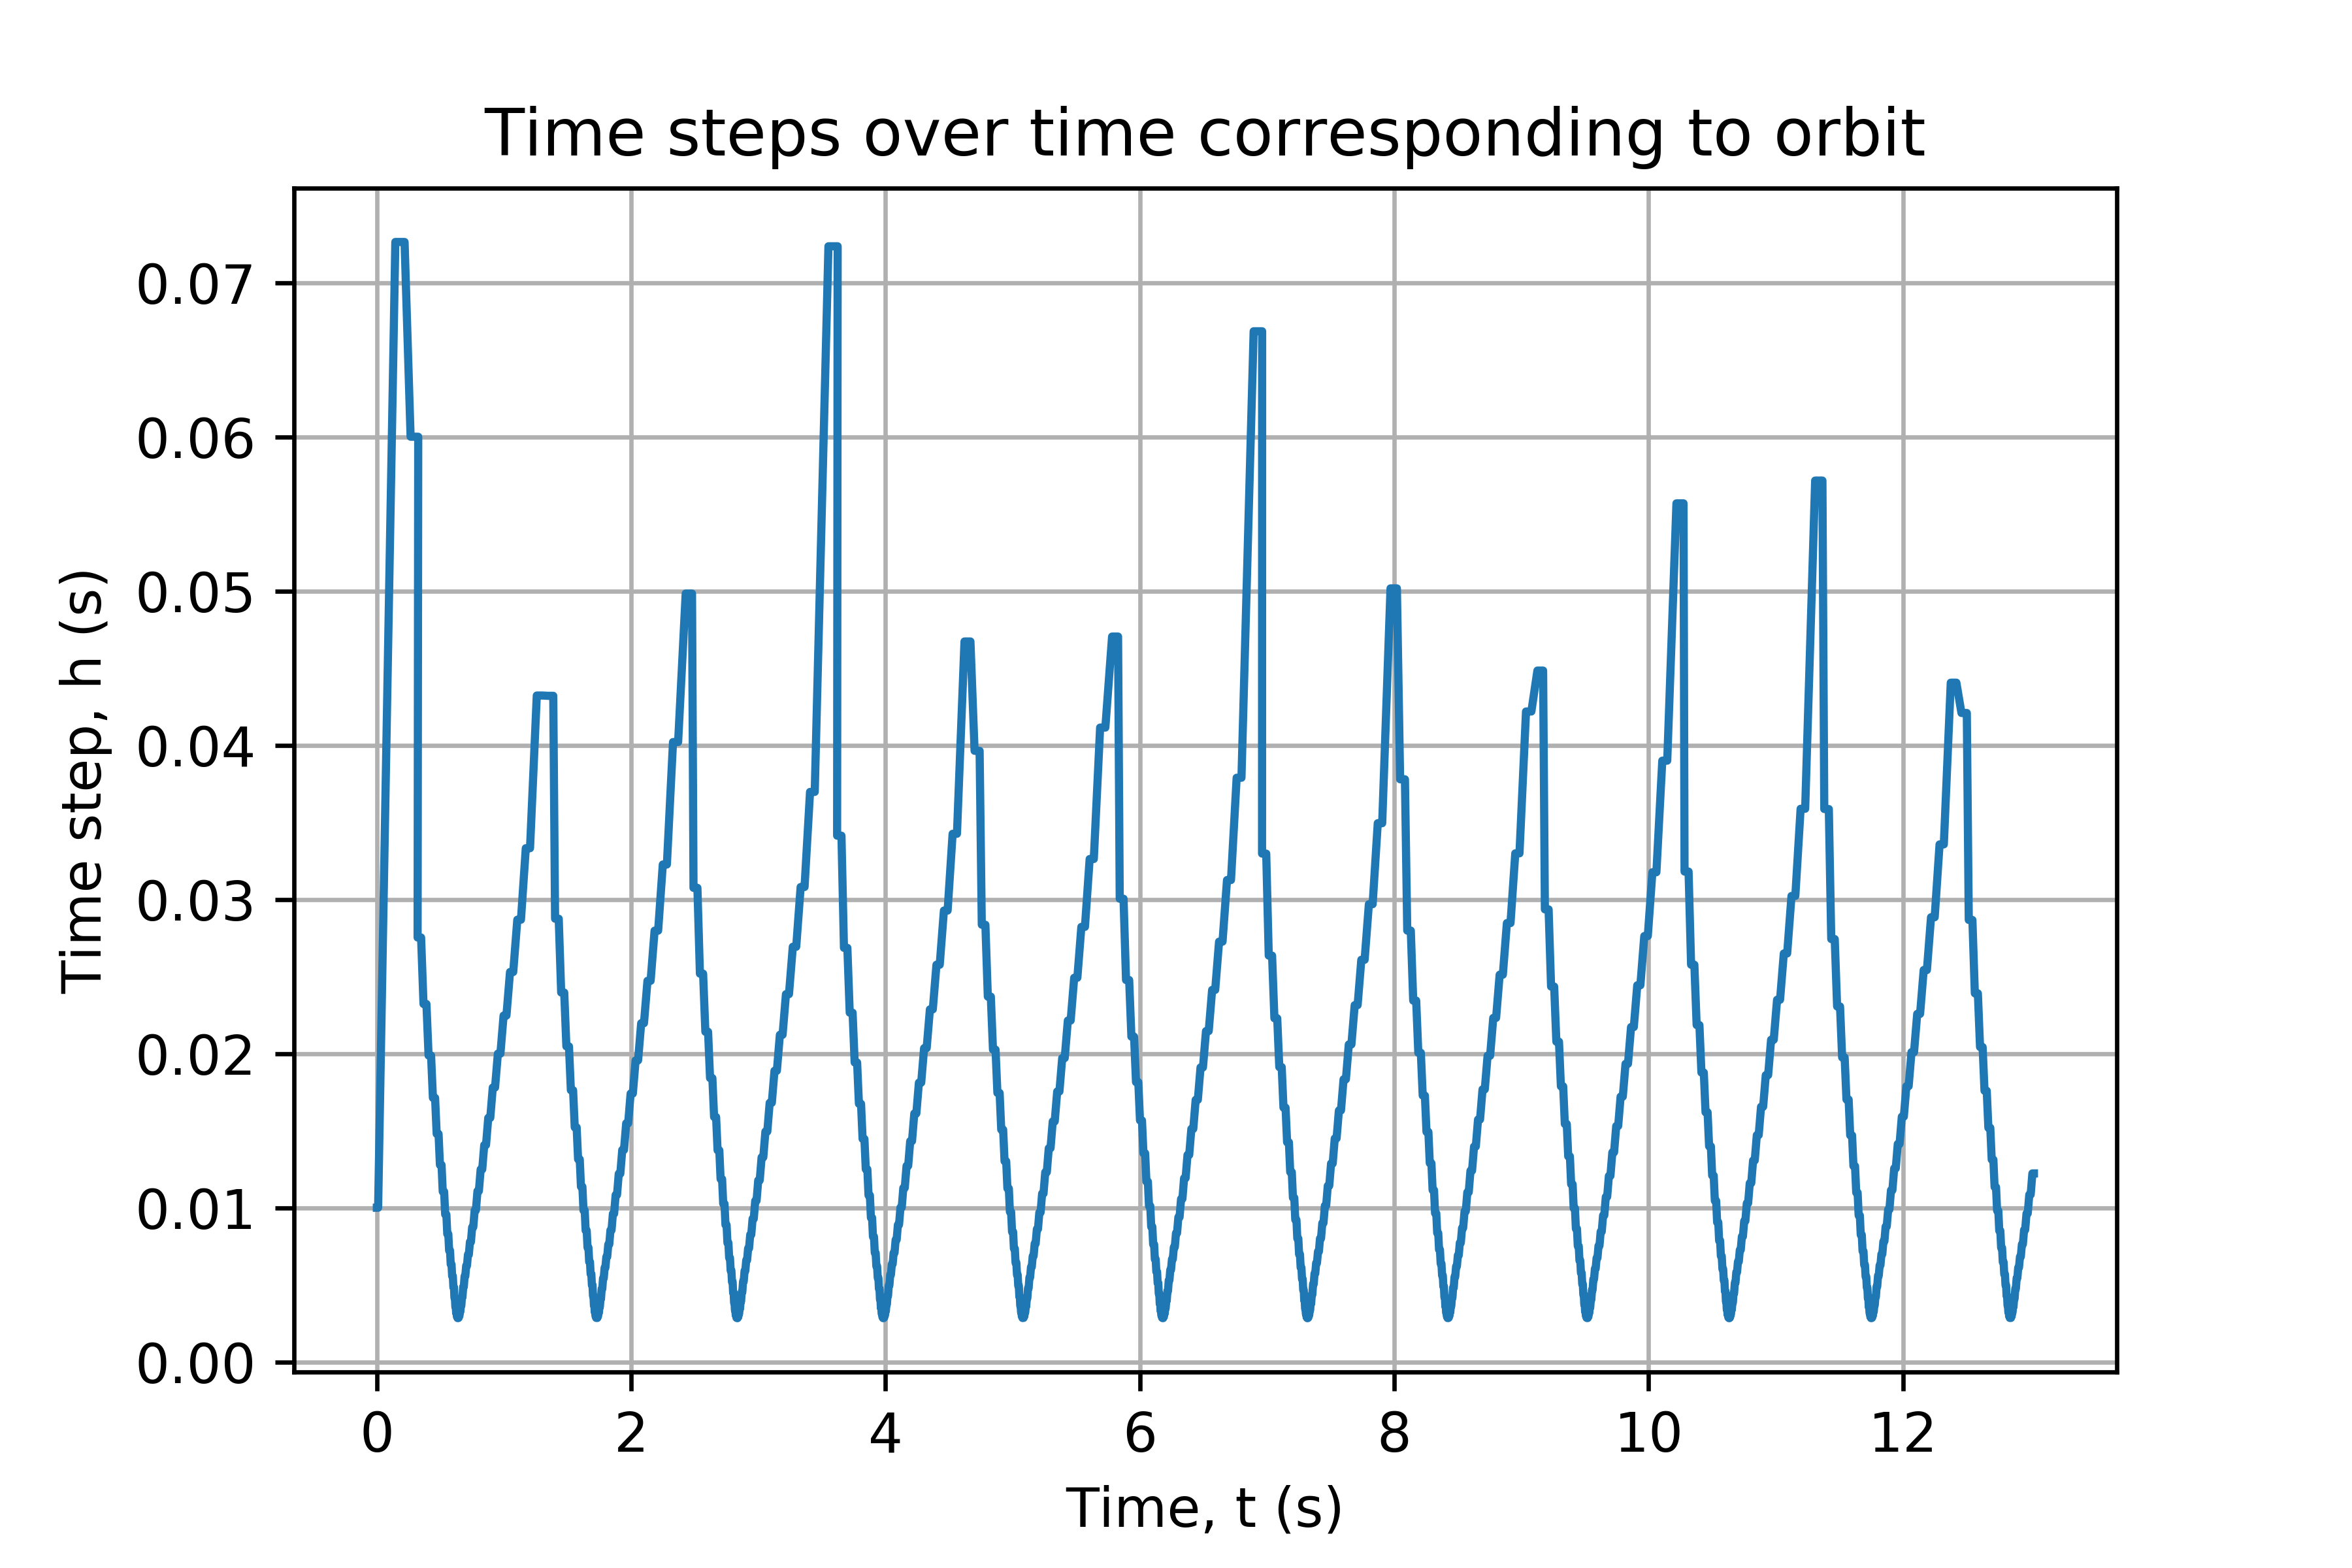
\includegraphics[width=0.8\textwidth]{../images/q1_orbit_step.png}
	\caption{Time step size over time in orbit corresponding to the solution of a ball bearing orbiting a rod in space attained using the 4th order Runge-Kutta method with an adaptive time step.}
	\label{fig:q1_c}
\end{figure}


\section{The Hydrogen Atom}

\subsection{Part b)}

We seek to use our program to compute the energies of the ground state and the first excited state (for $l=0$ and $l=1$), and observe the effects of changing various parameters on the accuracy of the computation.

The computed values of the energy for the first two excited states, along with the theoretical values, are displayed in table \ref{tab:2b_i}. These values were computed using the suggested parameter values of $h=0.002a$, $r_\infty=20a$ (where $a$ is the Bohr radius), and a target accuracy of $e/1000$, and we can see that the agreement with the theoretical values is quite good for $n=2, l=1$, is okay for $n=2, l=0$ and $n=1, l=0$.

\begin{table}[H]
	\centering
	\caption{Numerically calculated energy values of the ground state and first excited state of the hydrogen atom, along with the theoretical values. Program used suggested parameter values of $h=0.002a$, $r_\infty=20a$, and a target accuracy of $e/1000$.}
	\label{tab:2b_i}
	\begin{tabular}{c|c|c|c}
		$n$ & $l$ & Calculated $E$ (eV)  & Literature $E$ (eV) \\
		\hline
		1 & 0 & -13.5004889817 & -13.605693009 \\
		2 & 0 & -3.3878669497 & -3.40142325225 \\
		2 & 1 & -3.40127671989 & -3.40142325225 \\
	\end{tabular}
\end{table}

In table \ref{tab:2b_ii} we display the calculated values of the energy for the first three states for three different values of $r_\infty$ with fixed step size $h=0.002a$ and target accuracy of $e/1000$. As can be seen from the table, increasing the value of $r_\infty$ improves the accuracy of the solution in all cases, although the extent to which it does this depends on the particular energy level and angular momentum value, and in some cases (i.e. $n=1, l=0$ the observed improvements were negligible.

\begin{table}[H]
	\centering
	\caption{Numerically calculated energy values of the ground state and first excited state of the hydrogen atom, along with the theoretical values, for different values of $r_\infty$ with $h=0.002a$ and a target accuracy of $e/1000$.}
	\label{tab:2b_ii}
	\begin{tabular}{c|c|c|c|c|c}
		$n$ & $l$ & $r_\infty=10a$ &  $r_\infty=20a$ & $r_\infty=40a$ & Literature $E$ (eV) \\
		\hline
		1 & 0 & -13.5004703237 & -13.5004889817 & -13.5004917637 & -13.605693009 \\
		2 & 0 & -3.05116418764 & -3.3878669497 & -3.38822466074 &  -3.40142325225 \\
		2 & 1 & -3.23433299007 & -3.40127671989 & -3.40142286517 & -3.40142325225 \\
	\end{tabular}
\end{table}

In table \ref{tab:2b_iii} we display the calculated values of the energy for the first three states for three different values of $h$ with fixed $r_\infty=20a$ and target accuracy of $e/1000$. As can be seen from the table, the accuracy of the calculations invariably increases with a smaller step size, and this improvement seems to be better than that for an increase in the value of $r_\infty$, although it is difficult to compare these two things given that the size of the variations tested is different, and itself difficult to compare. 

\begin{table}[H]
	\centering
	\caption{Numerically calculated energy values of the ground state and first excited state of the hydrogen atom, along with the theoretical values, for different values of $h$ with $r_\infty=20a$ and a target accuracy of $e/1000$.}
	\label{tab:2b_iii}
	\begin{tabular}{c|c|c|c|c|c}
		$n$ & $l$ & $h = 0.02a$ & $h = 0.002a$ & $h = 0.0002a$ & Literature $E$ (eV) \\
		\hline
		1 & 0 & -12.7092157518 & -13.5004889817 & -13.5949027472 & -13.605693009 \\
		2 & 0 & -3.28576534849 & -3.3878669497 & -3.39972201792 & -3.40142325225 \\
		2 & 1 & -3.40126355429 & -3.40127671989 & -3.40127673348 & -3.40142325225 \\
	\end{tabular}
\end{table}

In table \ref{tab:2b_iiii} we display the calculated values of the energy for the first three states for three different values of the target accuracy and with $h=0.002a$ and $r_\infty=20a$. As can be seen from the table, changing the target accuracy does not seem to have a very big effect on the accuracy of the calculation. This seems surprising, but makes sense if we consider that the accuracy we are specifying is simply requiring the solution to get closer to the value to which it is converging, and if it is converging to the incorrect value then changing the ``accuracy'' will not actually make it more accurate.

\begin{table}[H]
	\centering
	\caption{Numerically calculated energy values of the ground state and first excited state of the hydrogen atom, along with the theoretical values, for different target accuracies with $h=0.002a$ and $r_\infty=20a$.}
	\label{tab:2b_iiii}
	\begin{tabular}{c|c|c|c|c|c}
		$n$ & $l$ & target$=e/100$ & target$=e/1000$ & target$=e/10000$ & Literature $E$ (eV) \\
		\hline
		1 & 0 & -13.5009218107 & -13.5004889875 & -13.5004919696 & -13.605693009 \\
		2 & 0 & -3.38784656151 & -3.38786638765 & -3.38786638765 & -3.40142325225 \\
		2 & 1 & -3.40120743963 & -3.40127648895 & -3.40127648895 & -3.40142325225 \\
	\end{tabular}
\end{table}

\subsection{Part d)}

We seek to produce plots of the normalized computed wavefunctions $R(r)$ for each of the energy levels from the previous section, and compare the graphs of the functions to those of the theoretical solutions to the differential equation.

Plots of the eigenfunctions for all three sets of $n$ and $l$ values are shown in figures \ref{fig:q2_d_n=1_l=0}-\ref{fig:q2_d_n=2_l=1}. In light of the discussion in part b), we used parameter values of $h=0.0002a$, $r_\infty=20a$, and target accuracy of  $e/1000$ to compute the wavefunctions. In all figures, both the computed and theoretical wavefunctions have been normalized. As can be seen from the figures, the overall agreement between the computed and theoretical functions on the breadth of the domain is very good; the only discernible discrepancies occur at the endpoint $r=0$.

In the case of both $n=1, l=0$ (figure \ref{fig:q2_d_n=1_l=0}) and $n=2, l=0$ (figure \ref{fig:q2_d_n=2_l=0}), we see that the theoretical wavefunction increases to infinity at r=0. However, we required the boundary condition that $R(0) = 0$ in the numerical solution, so the numerical solution satisfies this condition and then quickly jumps up to match the theoretical value and follows it pretty much exactly over the rest of the domain, with no visible discrepancies. Thus, ignoring this one predictable error of the numerical method, the shape and zero crossings of the numerically computed wave functions, for the tested energy levels, agree very well with those of the theoretical/analytically determined wave functions.

Note that in the case of $n=2, l=1$, displayed in figure \ref{fig:q2_d_n=2_l=1}, the wavefunction does actually satisfy our imposed boundary condition of $R(0) = 0$, and we see that the computed and analytic wavefunctions agree very well over the whole domain, as we would expect them to.

\begin{figure}[H]
	\centering
	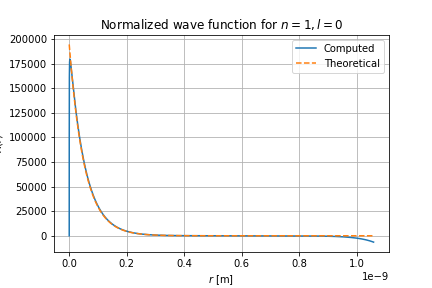
\includegraphics[width=0.8\textwidth]{../images/q2_d_n=1_l=0.png}
	\caption{Plot of computed and theoretical normalized wavefunction $R(r)$ for $n=1, l=0$.}
	\label{fig:q2_d_n=1_l=0}
\end{figure}

\begin{figure}[H]
	\centering
	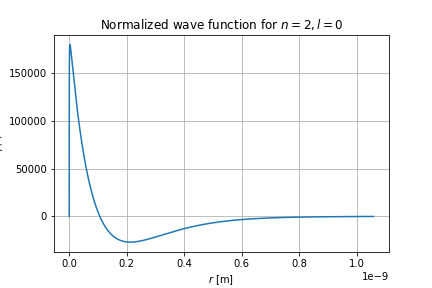
\includegraphics[width=0.8\textwidth]{../images/q2_d_n=2_l=0.png}
	\caption{Plot of computed and theoretical normalized wavefunction $R(r)$ for $n=2, l=0$.}
	\label{fig:q2_d_n=2_l=0}
\end{figure}

\begin{figure}[H]
	\centering
	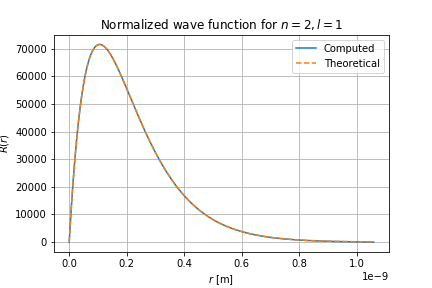
\includegraphics[width=0.8\textwidth]{../images/q2_d_n=2_l=1.png}
	\caption{Plot of computed and theoretical normalized wavefunction $R(r)$ for $n=2, l=1$.}
	\label{fig:q2_d_n=2_l=1}
\end{figure}

\end{document}